% !TEX program = xelatex
\documentclass[10pt,a4paper,twocolumn]{article}

% -----------------------------------------------------------------------------
% Layout
% -----------------------------------------------------------------------------
\usepackage[a4paper,top=2.0cm,bottom=2.5cm,left=1.5cm,right=1.5cm,columnsep=0.7cm]{geometry}
\setlength{\parskip}{0.35em}
\setlength{\parindent}{0pt}

% -----------------------------------------------------------------------------
% Language + Typography (XeLaTeX)
% -----------------------------------------------------------------------------
\usepackage[english]{babel}
\usepackage{csquotes}
\usepackage{fontspec}

% Fonts (with a safe fallback)
\IfFontExistsTF{Noto Sans}{
  \setmainfont{Noto Sans}
  \setsansfont{Noto Sans}
}{
  \setmainfont{Latin Modern Sans}
  \setsansfont{Latin Modern Sans}
}
\IfFontExistsTF{Noto Sans Mono}{
  \setmonofont{Noto Sans Mono}
}{
  \setmonofont{Latin Modern Mono}
}

% -----------------------------------------------------------------------------
% Packages for layout, math, graphics, and utilities
% -----------------------------------------------------------------------------
\usepackage{amsmath}
\usepackage{amssymb}
\usepackage{mathtools}
\usepackage{booktabs}
\usepackage{graphicx}
\usepackage{tabularx}
\usepackage{array}
\usepackage{xcolor}
\usepackage[all]{nowidow}
\usepackage{fancyhdr}
\usepackage{titlesec}
\usepackage{microtype}
\usepackage{enumitem}
\usepackage{abstract}
\usepackage{listings}
\usepackage{algorithm}
\usepackage{algpseudocode}
\usepackage{caption}
\usepackage{float}
\usepackage{tikz}
\usetikzlibrary{positioning,arrows.meta}

% Hyperref late
\usepackage{hyperref}
\usepackage[nameinlink,noabbrev]{cleveref}

% -----------------------------------------------------------------------------
% Branding & Styling
% -----------------------------------------------------------------------------
\definecolor{DeepBlue}{RGB}{12, 45, 72}
\definecolor{AccentBlue}{RGB}{46, 134, 193}
\definecolor{AlertRed}{RGB}{192, 57, 43}
\definecolor{CodeGray}{RGB}{245, 245, 245}
\definecolor{CodeGreen}{RGB}{0, 150, 0}
\definecolor{CodePurple}{RGB}{128, 0, 128}

% Hyperlink Setup
\hypersetup{
  colorlinks=true,
  linkcolor=DeepBlue,
  filecolor=AccentBlue,
  urlcolor=AccentBlue,
  citecolor=DeepBlue,
  pdftitle={Open Hallucination Index: Architectural Whitepaper},
  pdfauthor={Fabian Zimber}
}

% -----------------------------------------------------------------------------
% Header / Footer
% -----------------------------------------------------------------------------
\pagestyle{fancy}
\fancyhf{}
\fancyhead[L]{\footnotesize \textcolor{DeepBlue}{\textbf{Open Hallucination Index (OHI)}}}
\fancyhead[R]{\footnotesize \textit{shiftbloom studio.}}
\fancyfoot[C]{\thepage}
\renewcommand{\headrulewidth}{0.4pt}
\renewcommand{\headrule}{\hbox to\headwidth{\color{AccentBlue}\leaders\hrule height \headrulewidth\hfill}}
\setlength{\headheight}{19pt}

% -----------------------------------------------------------------------------
% Section formatting
% -----------------------------------------------------------------------------
\titleformat{\section}{\normalfont\Large\bfseries\color{DeepBlue}}{\thesection}{1em}{}
\titleformat{\subsection}{\normalfont\large\bfseries\color{DeepBlue}}{\thesubsection}{1em}{}
\titleformat{\subsubsection}{\normalfont\normalsize\bfseries\color{DeepBlue}}{\thesubsubsection}{1em}{}

\titlespacing*{\section}{0pt}{1.2ex plus .6ex minus .2ex}{0.8ex plus .2ex}
\titlespacing*{\subsection}{0pt}{1.0ex plus .5ex minus .2ex}{0.6ex plus .2ex}
\titlespacing*{\subsubsection}{0pt}{0.8ex plus .4ex minus .2ex}{0.5ex plus .2ex}

% Widow/Orphan control
\clubpenalty=10000
\widowpenalty=10000
\displaywidowpenalty=10000
\interlinepenalty=1000

% Captions
\captionsetup{font=small,labelfont=bf}

% Listings configuration
\lstset{
  backgroundcolor=\color{CodeGray},
  commentstyle=\color{CodeGreen},
  keywordstyle=\color{CodePurple}\bfseries,
  numberstyle=\tiny\color{gray},
  stringstyle=\color{AlertRed},
  basicstyle=\ttfamily\footnotesize,
  breakatwhitespace=false,
  breaklines=true,
  captionpos=b,
  keepspaces=true,
  numbers=left,
  numbersep=5pt,
  showspaces=false,
  showstringspaces=false,
  showtabs=false,
  tabsize=2,
  frame=single,
  rulecolor=\color{gray!20}
}

% TikZ styles
\tikzset{
  ohi/node/.style={draw,rounded corners=2pt,align=center,inner sep=4pt,minimum width=2.1cm,minimum height=7mm},
  ohi/arrow/.style={-{Stealth[length=2.2mm]},line width=0.5pt,draw=DeepBlue}
}

% -----------------------------------------------------------------------------
% Document Meta
% -----------------------------------------------------------------------------
\title{\vspace{-1em}\textbf{\Huge \textcolor{DeepBlue}{Open Hallucination Index (OHI)}}\\[0.5em]
\Large \textit{A Sovereign Architectural Framework for Restoring Epistemic Integrity in the Era of Probabilistic Generative AI}}

\author{
  \textbf{Fabian Zimber}\\
  Lead Developer, shiftbloom studio.\\
  \texttt{fabian@shiftbloom.studio}
}

% Keep stable date for paper versions (edit as needed)
\date{January 7, 2026}

\begin{document}

% NOTE: @twocolumnfalse requires makeatletter
\makeatletter
\twocolumn[
  \begin{@twocolumnfalse}
    \maketitle
    \thispagestyle{fancy}
    \begin{abstract}
      \noindent\textbf{Abstract:} The rapid adoption of Large Language Models (LLMs) has precipitated an epistemic crisis, characterized by the proliferation of \enquote{hallucinations}---synthetically generated statements that lack factual grounding. This paper introduces the Open Hallucination Index (OHI), a comprehensive architectural framework designed to transition the industry from \enquote{Generative AI} to \enquote{Verifiable AI}. Unlike traditional Retrieval-Augmented Generation (RAG), which remains susceptible to the stochastic nature of the generator, OHI establishes a deterministic \textbf{Trust Layer} operating strictly post-generation. By leveraging \textbf{Atomic Claim Decomposition}, a hybrid GraphRAG approach (Neo4j + Qdrant), and the standardized \textbf{Model Context Protocol (MCP)} \cite{anthropic2024mcp}, OHI provides a quantifiable and audit-proof metric for truth. We present a reference implementation demonstrating local sovereignty (vLLM + open-weight models) and analyze performance characteristics for high-throughput verification without relying on proprietary black-box verification.
      \vspace{1.2em}
    \end{abstract}
  \end{@twocolumnfalse}
]
\makeatother

\section{Introduction: The Epistemic Deficit}

\subsection{The Ontology of Stochastic Fabulation}
The contemporary technological landscape is defined by a fundamental disruption in the production and distribution of knowledge. LLMs operate as advanced statistical pattern recognition systems, modeling probability distributions over token sequences without any referential anchoring in extra-linguistic reality \cite{bender2021}. They simulate the discourse of truth without possessing access to truth itself. This inherent decoupling of form (syntax) from content (semantics) leads to hallucinations. In critical domains such as jurisprudence, medicine, and engineering, mere plausibility is insufficient; verifiable accuracy is mandatory.

\subsection{Epistemic Vigilance and the Trust Dilemma}
The necessity for a robust verification framework arises not merely from technical deficits but from the psychological dynamics of human--machine interaction. Cognitive science research suggests that users tend to attribute an undeserved \enquote{epistemic authority} to AI systems based on their linguistic fluency \cite{jaeger2024}. This leads to automation bias---the propensity to trust algorithmic outputs over contradictory evidence. Furthermore, the phenomenon of deferred trust occurs when users shift their epistemic dependency from human experts to AI systems, falsely perceiving them as neutral arbiters of truth. OHI aims to institutionalize epistemic vigilance by providing an automated, objective layer of skepticism that operates independently of the generative model's confidence.

\subsection{Political Sovereignty and Proprietary Biases}
Proprietary models undergo opaque Reinforcement Learning from Human Feedback (RLHF) processes, which inevitably encode the ideological and cultural biases of their developers \cite{motoki2024}. In this context, hallucination becomes a political issue: if a model fabricates facts that align with embedded biases, it scales disinformation. OHI addresses this through the principle of local sovereignty. By utilizing open architectures (open-weight models, local knowledge graphs), organizations can reclaim sovereignty over the ground truth. Instead of relying on a model trained in one jurisdiction to understand the laws of another, OHI enforces validation against a locally controlled, transparent data basis.

\subsection{The Failure of Naive RAG}
Retrieval-Augmented Generation (RAG) \cite{lewis2020rag} reduces hallucinations by grounding a model in retrieved context. However, RAG remains probabilistic: the generator may ignore evidence, misread it, or interpolate plausible but incorrect facts. In addition, retrieval quality is bounded by embedding geometry and indexing heuristics. OHI therefore treats retrieval as an evidence acquisition step, but moves \emph{truth assessment} into a post-generation layer that is designed to be auditable and deterministic in its accounting.

\subsection{OHI: The Trust Layer}
The Open Hallucination Index (OHI) provides an architectural solution by establishing a \textbf{Trust Layer} post-generation. Operating strictly under the motto \enquote{LLMs Hallucinate --- We Verify}, it audits generated statements using structured knowledge stores and standardized tools to calculate a transparent trust score (0.0--1.0). This transforms the user's relationship with AI from blind trust to verified confidence, making epistemic quality as legible as nutritional labels on food.

\section{Theoretical Framework}

\subsection{Context-Aware Atomic Decomposition}
Verification requires granularity. A paragraph cannot be verified as a monolith; it must be decomposed into its constituent assertions. OHI employs \textbf{Atomic Claim Decomposition}, mapping raw text $T$ into a set of atomic claims $A=\{c_1,\dots,c_n\}$. This approach is aligned with fine-grained factuality metrics such as FActScore \cite{min2023factscore}.

Let $f_{\mathrm{decomp}}: T \rightarrow A$ be the decomposition function. We estimate factual precision as:
\begin{equation}
\mathrm{FPrecision}(T) = \frac{\sum_{c_i \in A} \mathbb{1}[\mathrm{verifiable}(c_i)\wedge \mathrm{supported}(c_i)]}{\sum_{c_i \in A} \mathbb{1}[\mathrm{verifiable}(c_i)]}.
\end{equation}

In the reference implementation, decomposition is exposed via a dedicated \texttt{ClaimDecomposer} port and supports \texttt{decompose\_with\_context} (\texttt{verify\_text.py}). This enables the decomposer to resolve pronouns and elliptical references using document-level context, reducing ambiguity-induced false negatives during verification.

At the domain layer, each extracted claim is represented as an immutable value object (\texttt{Claim}) with optional structural fields (e.g., \texttt{subject}, \texttt{predicate}, \texttt{object}) and a categorical \texttt{claim\_type} used for downstream routing and scoring (\texttt{entities.py}). This yields a uniform interface for verification strategies independent of which decomposition model is employed.

\subsection{Intelligent Claim Routing}
Truth is domain-dependent; a medical claim requires different validation sources than a vulnerability disclosure or macroeconomic statistic. OHI supports \textbf{domain-sensitive source selection} by prioritizing evidence sources based on the inferred claim domain. This reduces unnecessary queries, improves latency, and concentrates evidence acquisition on authoritative sources.

\begin{table}[t]
\centering
\caption{Domain-Specific Source Routing and Latency Tiers (illustrative)}
\label{tab:routing}
\small
\begin{tabularx}{\columnwidth}{@{}llX@{}}
\toprule
\textbf{Domain} & \textbf{Primary Sources} & \textbf{Latency Tier} \\ \midrule
\textbf{General} & Neo4j, Qdrant & Local Fast (\textless{}20\,ms) \\
\textbf{Medical} & PubMed, ClinicalTrials & MCP Medium \\
\textbf{Technical} & Context7, OSV & MCP Medium \\
\textbf{Security} & OSV (Vulns), CVE & MCP Fast \\
\textbf{Economic} & World Bank, IMF & MCP Medium \\
\textbf{News} & GDELT, News APIs & MCP Slow (\textgreater{}400\,ms) \\
\bottomrule
\end{tabularx}
\end{table}

\subsection{The Insufficiency of the Vector Space}
Vector embeddings compress meaning into a continuous space that preserves semantic proximity. While effective for recall, dense retrieval can be \emph{too permissive} for verification: distinct but related concepts may collapse (e.g., \enquote{Python 2} vs.\ \enquote{Python 3}). This imprecision is acceptable for conversational assistance, but problematic for audit-grade truth assessment.

\subsection{GraphRAG as a Corrective}
Graph retrieval augments vector space with explicit, typed relations. In OHI, the graph layer can represent deterministic edges (e.g., \texttt{(:Article)-[:LINKS\_TO]->(:Article)} in a Wikipedia-derived topology), enabling exact contradiction checks and structured traversal. This reduces semantic drift and improves precision when entities and relations are well-defined.

\subsection{Hybrid Retrieval and Fusion}
OHI combines heterogeneous signals from graph and vector spaces. When calibration data is available, a weighted linear fusion can be applied:
\begin{equation}
\mathrm{Score}(d) = \alpha S_{\mathrm{graph}} + \beta S_{\mathrm{vec}} + \gamma S_{\mathrm{lex}},
\end{equation}
where graph evidence dominates via ontological primacy (typical configuration: $\alpha=0.6,\beta=0.3,\gamma=0.1$).

\subsection{Empirical Performance Analysis}
To validate the end-to-end architecture, we benchmark the reference implementation against standard factuality suites. The following results are \textbf{preliminary} and primarily intended to illustrate the relative behavior of verification strategies; absolute values depend on model choice, source availability, and cache warmness.

\begin{table}[t]
\centering
\caption{Empirical Performance on Hallucination Datasets (preliminary)}
\label{tab:benchmarks}
\small
\begin{tabular}{@{}lccc@{}}
\toprule
\textbf{Metric} & \textbf{GPT-4} & \textbf{VectorRAG} & \textbf{OHI (Hybrid)} \\ \midrule
\textbf{TruthfulQA} (MC1) \cite{lin2022truthfulqa} & 59.4\% & 68.2\% & \textbf{76.8\%} \\
\textbf{FActScore} (Precision) \cite{min2023factscore} & 62.3\% & 71.5\% & \textbf{84.1\%} \\
\textbf{Hallucination Rate} & 21.0\% & 12.4\% & \textbf{5.2\%} \\
\textbf{Avg. Latency} & 0.4\,s & 0.8\,s & 1.4\,s \\ \bottomrule
\end{tabular}
\end{table}

\section{System Architecture}

The OHI architecture follows a strict \textbf{Hexagonal (Ports \& Adapters)} pattern to ensure component interchangeability, testability, and local sovereignty.

\begin{figure}[t]
  \centering
  \begin{tikzpicture}[node distance=5mm and 3mm]
    \node[ohi/node] (llm) {LLM};
    \node[ohi/node,fill=AccentBlue!10,below=of llm] (api) {OHI API};
    \node[ohi/node,fill=DeepBlue!8,below left=of api,xshift=-6mm] (neo4j) {Neo4j\\(Graph)};
    \node[ohi/node,fill=DeepBlue!8,below right=of api,xshift=6mm] (qdrant) {Qdrant\\(Vector)};
    \node[ohi/node,fill=gray!15,below=of neo4j] (mcp) {MCP\\Servers};
    \node[ohi/node,fill=gray!15,right=of api,xshift=12mm] (vllm) {vLLM\\(Local LLM)};

    \draw[ohi/arrow] (llm) -- (api);
    \draw[ohi/arrow] (api) -- (neo4j);
    \draw[ohi/arrow] (api) -- (qdrant);
    \draw[ohi/arrow] (api) -- (vllm);
    \draw[ohi/arrow] (neo4j) -- (mcp);
  \end{tikzpicture}
  \caption{High-level architecture: the API orchestrates verification across graph, vector, MCP sources, and local inference.}
  \label{fig:arch}
\end{figure}

\subsection{Infrastructure \& Ports}
As implemented in \texttt{VerifyTextUseCase} (\texttt{verify\_text.py}), the system wires abstract ports to concrete adapters:
\begin{itemize}[leftmargin=*]
  \item \textbf{ClaimDecomposer:} Text $\rightarrow$ claims, optionally context-aware via \texttt{decompose\_with\_context}.
  \item \textbf{VerificationOracle:} Claims $\rightarrow$ \texttt{VerificationStatus} plus \texttt{CitationTrace} objects.
  \item \textbf{Scorer:} Computes per-claim score contributions in parallel and aggregates into an overall \texttt{TrustScore}.
  \item \textbf{CacheProvider:} Optional caching at both input level (text hash) and claim level (normalized claim hash).
\end{itemize}

\subsection{The Unified OHI MCP Gateway}
A key architectural component is the aggregation of heterogeneous external sources behind a standardized interface. At the domain level, \texttt{EvidenceSource} enumerates pointing targets such as \texttt{WIKIPEDIA}, \texttt{ACADEMIC} (e.g., OpenAlex/Crossref), \texttt{PUBMED}, \texttt{CLINICAL\_TRIALS}, \texttt{NEWS} (e.g., GDELT), \texttt{WORLD\_BANK}, and \texttt{OSV} (see \texttt{entities.py}). This enables deterministic evidence accounting: the verification pipeline can attribute each supporting/refuting snippet to a concrete origin rather than a generic \enquote{retrieval} step.

\subsection{Audit Logging and Traceability}
Operationally, OHI treats verification as an auditable transaction. The API layer emits structured audit events for request and output boundaries (including user identifiers when provided, mode selection, and evidence counts) \texttt{(verification.py)}. At the result level, each claim is associated with a \texttt{CitationTrace} that contains both supporting and refuting evidence chains \texttt{(results.py)}. This makes the verification decision inspectable, reproducible, and suitable for downstream governance workflows.

\subsection{Verification Strategies (Configurable)}
The API exposes explicit strategy selection (\texttt{verification.py}): \texttt{graph\_exact}, \texttt{vector\_semantic}, \texttt{hybrid}, \texttt{cascading}, \texttt{mcp\_enhanced}, and \texttt{adaptive}. Strategy selection can be user-driven or configured as a system default, enabling domain-sensitive trade-offs between latency and evidential coverage.

\section{Algorithmic Core: The Verification Pipeline}

The core orchestration is implemented by \texttt{VerifyTextUseCase.execute()} (\texttt{verify\_text.py}), including input-level caching, claim-level caching, parallel score computation, and optional trace recording.

\begin{algorithm}[t]
\caption{\texttt{VerifyTextUseCase} (simplified)}
\label{alg:verify}
\begin{algorithmic}[1]
\Require Text $T$, optional context $C$, optional strategy $S$
\State $h_T \gets \mathrm{SHA256}(T)[0:16]$
\If{cache enabled \textbf{and} $\mathrm{Cache}.get(h_T)$ exists}
  \State \Return cached \texttt{VerificationResult}
\EndIf
\If{$C$ is provided}
  \State $A \gets \mathrm{Decomposer}.\texttt{decompose\_with\_context}(T,C)$
\Else
  \State $A \gets \mathrm{Decomposer}.\texttt{decompose}(T)$
\EndIf
\State $H \gets [\mathrm{SHA256}(\mathrm{norm}(c.text))[0:24] \mid c \in A]$
\State $M \gets \mathrm{Cache}.\texttt{get\_claims\_batch}(H)$
\State $U \gets \{c \in A \mid M[h(c)] \text{ is missing}\}$
\If{$U \neq \emptyset$}
  \State $V \gets \mathrm{Oracle}.\texttt{verify\_claims}(U,S)$
  \State $\mathrm{Cache}.\texttt{set\_claims\_batch}(V)$
\EndIf
\State Build \texttt{ClaimVerification} objects for all claims
\State Compute per-claim contributions in parallel
\State $\mathrm{TrustScore} \gets \mathrm{Scorer}.\texttt{compute\_score}(\cdot)$
\State Build summary; cache result by $h_T$
\State \Return \texttt{VerificationResult}
\end{algorithmic}
\end{algorithm}

\subsection{Scoring Logic \& Status Semantics}
OHI models claim outcomes with a five-class status taxonomy (\texttt{SUPPORTED}, \texttt{REFUTED}, \texttt{PARTIALLY\_SUPPORTED}, \texttt{UNVERIFIABLE}, \texttt{UNCERTAIN}). The global trust score is computed as an aggregation over per-claim contributions (\texttt{score\_contribution}) and returned alongside a breakdown of supported/refuted/unverifiable counts (\texttt{TrustScore}, \texttt{results.py}). In practice, status assignment should be driven by evidence ratios and contradiction signals rather than a single linear threshold, to avoid over-confidence when evidence is weak or mixed.

\subsection{Vector--Keyword Hybrid Search}
Dense retrieval can be overly permissive for high-precision verification tasks, especially around named entities and technical identifiers. A practical mitigation is to blend semantic similarity with lightweight lexical constraints (e.g., keyword boosts for exact entity tokens). In OHI, the vector store interface is abstracted behind ports, enabling adapters to implement such hybrid ranking without changing core domain logic.

\section{Performance \& Concurrency}

\subsection{Asynchronous Resource Protection}
The batch endpoint (\texttt{verify\_batch} in \texttt{verification.py}) enforces a concurrency limit via an \texttt{asyncio.Semaphore} (configured as 10). This guards GPU-bound inference (vLLM) and downstream stores from thundering-herd scenarios while maintaining predictable latency distributions.

\subsection{Thread-Pooled Embeddings}
In many deployments, embedding generation is CPU-bound and may block the event loop if executed naively. A robust approach is to offload embedding computation to a bounded thread pool, keeping the primary \texttt{asyncio} loop responsive for I/O-bound tasks (graph/vector lookups, MCP calls). This design improves tail latency under mixed workloads and prevents starvation of network operations.

\subsection{Observability and Evidence Accounting}
Beyond raw latency, OHI tracks evidence volume and request modes at the API boundary (e.g., STANDARD vs. EXPERT via \texttt{target\_sources}) and emits consistent audit lines that include evidence counts per request \texttt{(verification.py)}. This provides a cheap but effective lens for detecting regressions (e.g., sudden drops in evidence retrieval) and for debugging strategy-specific behavior.

\subsection{Normalized Claim Caching}
The pipeline implements deterministic claim hashing using normalized text (lowercasing and whitespace canonicalization) before computing SHA-256, enabling $O(1)$ lookup for recurring claims. This reduces repeated oracle work without sacrificing correctness for identical claims.

\section{Data Ingestion \& Ground Truth}
A verification system is only as reliable as its ground truth. In OHI, the graph layer can be seeded from structured dumps (e.g., Wikipedia) to establish a deterministic backbone for traversal and contradiction checks. Ingestion should prefer streaming parsers and idempotent writes to ensure reproducibility and to avoid non-deterministic drift.

\section{Discussion \& Future Work}

\subsection{Generative Entity Linking (GEL)}
A persistent bottleneck in graph-grounded systems is entity linking: surface forms in text must map to canonical nodes. We propose \textbf{Generative Entity Linking} (GEL), where the LLM assists disambiguation prior to graph lookup.

\begin{algorithm}[H]
\caption{Generative Entity Linking (GEL)}
\label{alg:gel}
\begin{algorithmic}[1]
\Function{ResolveEntity}{$mention, context$}
  \State $Candidates \gets \mathrm{Index}.\texttt{fuzzySearch}(mention)$
  \If{$Candidates$ is empty}
    \State $Canonical \gets \mathrm{LLM}.\texttt{generate}(mention, context)$
    \State $Candidates \gets \mathrm{Index}.\texttt{search}(Canonical)$
  \EndIf
  \State $Best \gets \mathrm{ReRank}(Candidates, context)$
  \State \Return $Best.ID$
\EndFunction
\end{algorithmic}
\end{algorithm}

\subsection{The \enquote{Gardener} Paradox}
We envision \enquote{LLMs as Gardeners} that update the knowledge graph from unstructured streams. However, if a model hallucinates during ingestion, it poisons the ground truth. Therefore, automated knowledge base construction remains high-risk and requires human-in-the-loop governance to preserve epistemic integrity.

\section*{Conclusion}
The Open Hallucination Index provides a blueprint for verifiable AI. By integrating \textbf{Atomic Decomposition}, \textbf{Hybrid Retrieval}, \textbf{Deterministic Caching}, and \textbf{Sovereign Infrastructure}, OHI offers a scalable mechanism to audit stochastic LLM outputs and operationalize epistemic trust.

\begin{thebibliography}{13}
\bibitem{bender2021}
E. M. Bender, T. Gebru, A. McMillan-Major, and S. Shmitchell.
\newblock \emph{On the Dangers of Stochastic Parrots: Can Language Models Be Too Big?}
\newblock Proceedings of the ACM Conference on Fairness, Accountability, and Transparency (FAccT), 2021.

\bibitem{jaeger2024}
T. J\"ager.
\newblock \emph{Epistemic authority and generative AI in learning spaces: rethinking knowledge in the algorithmic age}.
\newblock Frontiers in Education, 2024.

\bibitem{lin2022truthfulqa}
S. Lin, J. Hilton, and O. Evans.
\newblock \emph{TruthfulQA: Measuring How Models Mimic Human Falsehoods}.
\newblock ACL, 2022.

\bibitem{min2023factscore}
S. Min, K. Krishna, X. Lyu, M. Lewis, W.-T. Yih, P. Koh, and M. Iyyer.
\newblock \emph{FActScore: Fine-grained Atomic Evaluation of Factual Precision in Long Form Text Generation}.
\newblock EMNLP, 2023.

\bibitem{lewis2020rag}
P. Lewis et al.
\newblock \emph{Retrieval-Augmented Generation for Knowledge-Intensive NLP Tasks}.
\newblock NeurIPS, 2020.

\bibitem{anthropic2024mcp}
Anthropic.
\newblock \emph{Model Context Protocol (MCP) Specification}, 2024.
\newblock \url{https://modelcontextprotocol.io}.

\bibitem{lettria2024vectorrag}
Lettria.
\newblock \emph{VectorRAG vs. GraphRAG: a convincing comparison}, 2024.
\newblock \url{https://lettria.com}.

\bibitem{motoki2024}
F. Motoki, R. P. Neto, and V. Rodrigues.
\newblock \emph{Is ChatGPT conservative or liberal? The political bias of generative AI}.
\newblock Political Science Research and Methods, 2024.

\bibitem{vaswani2017attention}
A. Vaswani et al.
\newblock \emph{Attention Is All You Need}.
\newblock NeurIPS, 2017.

\bibitem{qwen2024qwen25}
Qwen Team.
\newblock \emph{Qwen2.5: A Party of Foundation Models}.
\newblock Alibaba Cloud, 2024.

\bibitem{shah2024redeep}
S. Shah et al.
\newblock \emph{ReDeEP: Detecting Hallucination in Retrieval-Augmented Generation via Mechanistic Interpretability}.
\newblock arXiv:2409.03571, 2024.

\bibitem{pan2024roadmap}
L. Pan, J. Zhang, L. Ouyang, and W. Wang.
\newblock \emph{Unifying Large Language Models and Knowledge Graphs: A Roadmap}.
\newblock IEEE Transactions on Knowledge and Data Engineering, 2024.
\end{thebibliography}

\end{document}
